%auto-ignore
\ifx\compilefullpaper\undefined  
\documentclass[11pt]{article}
%auto-ignore
\usepackage{fullpage}
\usepackage{amsfonts, amssymb, amsmath, amsthm}
\usepackage{latexsym}
\usepackage[tracking=smallcaps]{microtype}	% for an arXiv submission, set \pdfoutput=1 near the top so it uses pdflatex
\usepackage{url}
\usepackage{color}
\definecolor{DarkGray}{rgb}{0.1,0.1,0.5}
\usepackage[colorlinks=true,breaklinks, linkcolor=black,citecolor=black,urlcolor=DarkGray]{hyperref}	% linkcolor=blue,citecolor=blue,urlcolor=blue %DarkGray

\usepackage{graphicx}
\usepackage[tight, TABBOTCAP]{subfigure}
%\usepackage{cancel}
%\usepackage{multirow}
%\usepackage[small]{caption}	%% caption package is useful for allowing line breaks within figure captions

%\usepackage{import}
%\usepackage{longtable}
%\usepackage{booktabs}
%\usepackage{ltxtable}
%\usepackage{rotating}	%% rotating package defines sideways environment

%\usepackage{calc}	%% The calc package reimplements the LaTeX commands \setcounter, ..., so that these commands accept an infix notation expression.

%\let\oldbibliography\thebibliography
%\renewcommand{\thebibliography}[1]{%
%  \oldbibliography{#1}%
%  \setlength{\itemsep}{.25pt}%
%}

%\usepackage[letterpaper]{geometry}		\geometry{includefoot,verbose,nohead,tmargin=1in,bmargin=.75in,lmargin=1.5in,rmargin=1in}
%\setlength{\parindent}{0.25in} \setlength{\parskip}{6pt}	\renewcommand{\baselinestretch}{1.66}	% stretch things out
%\def\ssp{\def\baselinestretch{1.0}\large\normalsize}	% single-space references

\def\place #1#2#3{\mspace{#2}\makebox[0pt]{\raisebox{#3}{#1}}\mspace{-#2}}	% the second argument should be in mu, and the third argument in pt

%%    Q-circuit version 2
%    Copyright (C) 2004  Steve Flammia & Bryan Eastin
%    Last modified on: 9/16/2011
%
%    This program is free software; you can redistribute it and/or modify
%    it under the terms of the GNU General Public License as published by
%    the Free Software Foundation; either version 2 of the License, or
%    (at your option) any later version.
%
%    This program is distributed in the hope that it will be useful,
%    but WITHOUT ANY WARRANTY; without even the implied warranty of
%    MERCHANTABILITY or FITNESS FOR A PARTICULAR PURPOSE.  See the
%    GNU General Public License for more details.
%
%    You should have received a copy of the GNU General Public License
%    along with this program; if not, write to the Free Software
%    Foundation, Inc., 59 Temple Place, Suite 330, Boston, MA  02111-1307  USA

% Thanks to the Xy-pic guys, Kristoffer H Rose, Ross Moore, and Daniel Müllner,
% for their help in making Qcircuit work with Xy-pic version 3.8.  
% Thanks also to Dave Clader, Andrew Childs, Rafael Possignolo, Tyson Williams,
% Sergio Boixo, Cris Moore, Jonas Anderson, and Stephan Mertens for helping us test 
% and/or develop the new version.

\usepackage{xy}
\xyoption{matrix}
\xyoption{frame}
\xyoption{arrow}
\xyoption{arc}

\usepackage{ifpdf}
\ifpdf
\else
\PackageWarningNoLine{Qcircuit}{Qcircuit is loading in Postscript mode.  The Xy-pic options ps and dvips will be loaded.  If you wish to use other Postscript drivers for Xy-pic, you must modify the code in Qcircuit.tex}
%    The following options load the drivers most commonly required to
%    get proper Postscript output from Xy-pic.  Should these fail to work,
%    try replacing the following two lines with some of the other options
%    given in the Xy-pic reference manual.
\xyoption{ps}
\xyoption{dvips}
\fi

% The following resets Xy-pic matrix alignment to the pre-3.8 default, as
% required by Qcircuit.
\entrymodifiers={!C\entrybox}

\newcommand{\bra}[1]{{\left\langle{#1}\right\vert}}
\newcommand{\ket}[1]{{\left\vert{#1}\right\rangle}}
    % Defines Dirac notation. %7/5/07 added extra braces so that the commands will work in subscripts.
\newcommand{\qw}[1][-1]{\ar @{-} [0,#1]}
    % Defines a wire that connects horizontally.  By default it connects to the object on the left of the current object.
    % WARNING: Wire commands must appear after the gate in any given entry.
\newcommand{\qwx}[1][-1]{\ar @{-} [#1,0]}
    % Defines a wire that connects vertically.  By default it connects to the object above the current object.
    % WARNING: Wire commands must appear after the gate in any given entry.
\newcommand{\cw}[1][-1]{\ar @{=} [0,#1]}
    % Defines a classical wire that connects horizontally.  By default it connects to the object on the left of the current object.
    % WARNING: Wire commands must appear after the gate in any given entry.
\newcommand{\cwx}[1][-1]{\ar @{=} [#1,0]}
    % Defines a classical wire that connects vertically.  By default it connects to the object above the current object.
    % WARNING: Wire commands must appear after the gate in any given entry.
\newcommand{\gate}[1]{*+<.6em>{#1} \POS ="i","i"+UR;"i"+UL **\dir{-};"i"+DL **\dir{-};"i"+DR **\dir{-};"i"+UR **\dir{-},"i" \qw}
    % Boxes the argument, making a gate.
\newcommand{\meter}{*=<1.8em,1.4em>{\xy ="j","j"-<.778em,.322em>;{"j"+<.778em,-.322em> \ellipse ur,_{}},"j"-<0em,.4em>;p+<.5em,.9em> **\dir{-},"j"+<2.2em,2.2em>*{},"j"-<2.2em,2.2em>*{} \endxy} \POS ="i","i"+UR;"i"+UL **\dir{-};"i"+DL **\dir{-};"i"+DR **\dir{-};"i"+UR **\dir{-},"i" \qw}
    % Inserts a measurement meter.
    % In case you're wondering, the constants .778em and .322em specify
    % one quarter of a circle with radius 1.1em.
    % The points added at + and - <2.2em,2.2em> are there to strech the
    % canvas, ensuring that the size is unaffected by erratic spacing issues
    % with the arc.
\newcommand{\measure}[1]{*+[F-:<.9em>]{#1} \qw}
    % Inserts a measurement bubble with user defined text.
\newcommand{\measuretab}[1]{*{\xy*+<.6em>{#1}="e";"e"+UL;"e"+UR **\dir{-};"e"+DR **\dir{-};"e"+DL **\dir{-};"e"+LC-<.5em,0em> **\dir{-};"e"+UL **\dir{-} \endxy} \qw}
    % Inserts a measurement tab with user defined text.
\newcommand{\measureD}[1]{*{\xy*+=<0em,.1em>{#1}="e";"e"+UR+<0em,.25em>;"e"+UL+<-.5em,.25em> **\dir{-};"e"+DL+<-.5em,-.25em> **\dir{-};"e"+DR+<0em,-.25em> **\dir{-};{"e"+UR+<0em,.25em>\ellipse^{}};"e"+C:,+(0,1)*{} \endxy} \qw}
    % Inserts a D-shaped measurement gate with user defined text.
\newcommand{\multimeasure}[2]{*+<1em,.9em>{\hphantom{#2}} \qw \POS[0,0].[#1,0];p !C *{#2},p \drop\frm<.9em>{-}}
    % Draws a multiple qubit measurement bubble starting at the current position and spanning #1 additional gates below.
    % #2 gives the label for the gate.
    % You must use an argument of the same width as #2 in \ghost for the wires to connect properly on the lower lines.
\newcommand{\multimeasureD}[2]{*+<1em,.9em>{\hphantom{#2}} \POS [0,0]="i",[0,0].[#1,0]="e",!C *{#2},"e"+UR-<.8em,0em>;"e"+UL **\dir{-};"e"+DL **\dir{-};"e"+DR+<-.8em,0em> **\dir{-};{"e"+DR+<0em,.8em>\ellipse^{}};"e"+UR+<0em,-.8em> **\dir{-};{"e"+UR-<.8em,0em>\ellipse^{}},"i" \qw}
    % Draws a multiple qubit D-shaped measurement gate starting at the current position and spanning #1 additional gates below.
    % #2 gives the label for the gate.
    % You must use an argument of the same width as #2 in \ghost for the wires to connect properly on the lower lines.
\newcommand{\control}{*!<0em,.025em>-=-<.2em>{\bullet}}
    % Inserts an unconnected control.
\newcommand{\controlo}{*+<.01em>{\xy -<.095em>*\xycircle<.19em>{} \endxy}}
    % Inserts a unconnected control-on-0.
\newcommand{\ctrl}[1]{\control \qwx[#1] \qw}
    % Inserts a control and connects it to the object #1 wires below.
\newcommand{\ctrlo}[1]{\controlo \qwx[#1] \qw}
    % Inserts a control-on-0 and connects it to the object #1 wires below.
\newcommand{\targ}{*+<.02em,.02em>{\xy ="i","i"-<.39em,0em>;"i"+<.39em,0em> **\dir{-}, "i"-<0em,.39em>;"i"+<0em,.39em> **\dir{-},"i"*\xycircle<.4em>{} \endxy} \qw}
    % Inserts a CNOT target.
\newcommand{\qswap}{*=<0em>{\times} \qw}
    % Inserts half a swap gate.
    % Must be connected to the other swap with \qwx.
\newcommand{\multigate}[2]{*+<1em,.9em>{\hphantom{#2}} \POS [0,0]="i",[0,0].[#1,0]="e",!C *{#2},"e"+UR;"e"+UL **\dir{-};"e"+DL **\dir{-};"e"+DR **\dir{-};"e"+UR **\dir{-},"i" \qw}
    % Draws a multiple qubit gate starting at the current position and spanning #1 additional gates below.
    % #2 gives the label for the gate.
    % You must use an argument of the same width as #2 in \ghost for the wires to connect properly on the lower lines.
\newcommand{\ghost}[1]{*+<1em,.9em>{\hphantom{#1}} \qw}
    % Leaves space for \multigate on wires other than the one on which \multigate appears.  Without this command wires will cross your gate.
    % #1 should match the second argument in the corresponding \multigate.
\newcommand{\push}[1]{*{#1}}
    % Inserts #1, overriding the default that causes entries to have zero size.  This command takes the place of a gate.
    % Like a gate, it must precede any wire commands.
    % \push is useful for forcing columns apart.
    % NOTE: It might be useful to know that a gate is about 1.3 times the height of its contents.  I.e. \gate{M} is 1.3em tall.
    % WARNING: \push must appear before any wire commands and may not appear in an entry with a gate or label.
\newcommand{\gategroup}[6]{\POS"#1,#2"."#3,#2"."#1,#4"."#3,#4"!C*+<#5>\frm{#6}}
    % Constructs a box or bracket enclosing the square block spanning rows #1-#3 and columns=#2-#4.
    % The block is given a margin #5/2, so #5 should be a valid length.
    % #6 can take the following arguments -- or . or _\} or ^\} or \{ or \} or _) or ^) or ( or ) where the first two options yield dashed and
    % dotted boxes respectively, and the last eight options yield bottom, top, left, and right braces of the curly or normal variety.  See the Xy-pic reference manual for more options.
    % \gategroup can appear at the end of any gate entry, but it's good form to pick either the last entry or one of the corner gates.
    % BUG: \gategroup uses the four corner gates to determine the size of the bounding box.  Other gates may stick out of that box.  See \prop.

\newcommand{\rstick}[1]{*!L!<-.5em,0em>=<0em>{#1}}
    % Centers the left side of #1 in the cell.  Intended for lining up wire labels.  Note that non-gates have default size zero.
\newcommand{\lstick}[1]{*!R!<.5em,0em>=<0em>{#1}}
    % Centers the right side of #1 in the cell.  Intended for lining up wire labels.  Note that non-gates have default size zero.
\newcommand{\ustick}[1]{*!D!<0em,-.5em>=<0em>{#1}}
    % Centers the bottom of #1 in the cell.  Intended for lining up wire labels.  Note that non-gates have default size zero.
\newcommand{\dstick}[1]{*!U!<0em,.5em>=<0em>{#1}}
    % Centers the top of #1 in the cell.  Intended for lining up wire labels.  Note that non-gates have default size zero.
\newcommand{\Qcircuit}{\xymatrix @*=<0em>}
    % Defines \Qcircuit as an \xymatrix with entries of default size 0em.
\newcommand{\link}[2]{\ar @{-} [#1,#2]}
    % Draws a wire or connecting line to the element #1 rows down and #2 columns forward.
\newcommand{\pureghost}[1]{*+<1em,.9em>{\hphantom{#1}}}
    % Same as \ghost except it omits the wire leading to the left. 

%\renewcommand{\measureD}[1]{*{\xy*+=+<.5em>{\vphantom{\rule{0em}{.1em}#1}}*\cir{r_l};p\save*!R{#1} \restore\save+UC;+UC-<.15em,0em>*!R{\hphantom{#1}}+L **\dir{-} \restore\save+DC;+DC-<.15em,0em>*!R{\hphantom{#1}}+L **\dir{-} \restore\POS+UC-<.1em,0em>*!R{\hphantom{#1}}+L;+DC-<.15em,0em>*!R{\hphantom{#1}}+L **\dir{-} \endxy} \qw}
\newcommand{\redcontrol}{*!<0em,.025em>-=-{\color{red}\bullet\color{black}}}
\newcommand{\redqwx}[1][-1]{\color{red}\ar @{-} [#1,0]\color{black}}
\newcommand{\redctrl}[1]{\redcontrol \redqwx[#1] \qw}
\newcommand{\redtarg}{*!<0em,.019em>=<.79em,.68em>{\color{red}\xy {<0em,0em>*{} \ar @{ - } +<.4em,0em> \ar @{ - } -<.4em,0em> \ar @{ - } +<0em,.36em> \ar @{ - } -<0em,.36em>},<0em,-.019em>*+<.8em>\frm{o}\endxy} \color{black}\qw}

\newcommand{\bra}[1]{{\langle#1|}}
\newcommand{\ket}[1]{{|#1\rangle}}
\newcommand{\braket}[2]{{\langle#1|#2\rangle}}
\newcommand{\ketbra}[2]{{\ket{#1}\!\bra{#2}}}
\newcommand{\lbra}[1]{{\bra{\overline{#1}}}}
\newcommand{\lket}[1]{{\ket{\overline{#1}}}}
\newcommand{\abs}[1]{{\lvert #1\rvert}}	% since the delimiters do not scale, it might be a good idea to add a dummy {} at the end, so \abs{big expression}^2 has the superscript at a low height
\newcommand{\bigabs}[1]{{\big\lvert #1\big\rvert}}
\newcommand{\Bigabs}[1]{{\Big\lvert #1\Big\rvert}}

\newcommand{\norm}[1]{{\| #1 \|}}
\newcommand{\bignorm}[1]{{\big\| #1 \big\|}}
\newcommand{\Bignorm}[1]{{\Big\| #1 \Big\|}}
\newcommand{\Biggnorm}[1]{{\Bigg\| #1 \Bigg\|}}
%\newcommand{\trnorm}[1]{{\norm{#1}_{\mathrm{tr}}}}
\newcommand{\trnorm}[1]{{\| #1 \|_{\mathrm{tr}}}}
\newcommand{\bigtrnorm}[1]{{\bigl\| #1 \bigr\|_{\mathrm{tr}}}}	% by not calling \bignorm, the subscript height is independent of the argument
\newcommand{\Bigtrnorm}[1]{{\Bigl\| #1 \Bigr\|_{\mathrm{tr}}}}
\newcommand{\Biggtrnorm}[1]{{\Biggl\| #1 \Biggr\|_{\mathrm{tr}}}}

\newcommand{\eps}{{\epsilon}}
\newcommand{\binomial}[2]{\ensuremath{\left(\begin{smallmatrix}#1 \\ #2 \end{smallmatrix}\right)}}
\newcommand{\fastmatrix}[1]{\left(\begin{smallmatrix}#1\end{smallmatrix}\right)}
\newcommand{\smatrx}[1]{\ensuremath{\left(\begin{smallmatrix}#1\end{smallmatrix}\right)}}
\newcommand{\matrx}[1]{\ensuremath{\left(\begin{matrix}#1\end{matrix}\right)}}
\DeclareMathOperator{\Ex}{\operatorname{E}}
\DeclareMathOperator{\Tr}{\operatorname{Tr}}

\def\tensor {\otimes}
\def\adjoint{\dagger} %{*}

\def\A {{\mathcal A}}
\def\B {{\mathcal B}}
\def\C {{\bf C}}
\def\D {{\mathcal D}}
\def\E {{\mathcal E}}
\def\F {{\mathcal F}}
\def\G {{\mathcal G}}
\def\H {{\mathcal H}}
\let\Lstroke\L	\def\L {{\mathcal L}}		
\def\N {{\bf N}}
\def\cP {{\mathcal P}}
\def\R {{\bf R}}
\def\S {{\mathcal S}}
\def\U {{\mathcal U}}
\def\V {{\mathcal V}}

%% Complexity classes: 
\renewcommand{\P}{\ensuremath{\mathsf{P}}}%{{\mathcal{NP}}}
\newcommand{\NP}{\ensuremath{\mathsf{NP}}}%{{\mathcal{NP}}}
\newcommand{\IP}{\ensuremath{\mathsf{IP}}}%{{\mathcal{NP}}}
\newcommand{\PSPACE}{\ensuremath{\mathsf{PSPACE}}}%{{\mathcal{NP}}}
\newcommand{\BQP}{\ensuremath{\mathsf{BQP}}}%{{\mathcal{BQP}}}
\newcommand{\EXP}{\ensuremath{\mathsf{EXP}}}%{{\mathcal{NP}}}
\newcommand{\NEXP}{\ensuremath{\mathsf{NEXP}}}%{{\mathcal{NP}}}
\newcommand{\QIP}{\ensuremath{\mathsf{QIP}}}%{{\mathcal{NP}}}
\newcommand{\QMIP}{\ensuremath{\mathsf{QMIP}}}%{{\mathcal{NP}}}
\newcommand{\MIP}{\ensuremath{\mathsf{MIP}}}%{{\mathcal{NP}}}

\DeclareMathOperator{\Span}{\operatorname{Span}}
\DeclareMathOperator{\Range}{\operatorname{Range}}
\DeclareMathOperator{\Kernel}{\operatorname{Ker}}
\DeclareMathOperator{\poly}{\operatorname{poly}}
\DeclareMathOperator{\qpoly}{\operatorname{qpoly}}
\DeclareMathOperator{\rank}{\operatorname{rank}}
\newcommand{\identity}{\ensuremath{\boldsymbol{1}}} %\mathbb{I}
\newcommand{\Id}{\identity} 
\DeclareMathOperator{\CNOT}{\operatorname{CNOT}}
\DeclareMathOperator{\SWAP}{\operatorname{SWAP}}

%\newtheorem*{maintheorem}{Main Theorem}

\newcommand{\hugelpar}[1]{\left(\vbox to #1{}\right.}
\newcommand{\hugerpar}[1]{\left.\vbox to #1{}\right)}
\newcounter{sprows}
\newcounter{spcols}
\newlength{\spheight}
\newlength{\spraise}
\newcommand{\spleft}[2][0pt]{\multirow{\value{sprows}}{*}{%
	\vbox to \spraise{\vss\hbox{$#2 \hugelpar{\spheight}\hskip -#1$}\vss}}}
\newcommand{\spright}[2][0pt]{\multirow{\value{sprows}}{*}{%
	\vbox to \spraise{\vss\hbox{\hskip -#1 $\hugerpar{\spheight} #2$}\vss}}}

\newcommand{\comment}[1]{\emph{\color{blue}Comment:\color{black} #1}} % use for simply removing comments
\newlength{\commentslength}
\newcommand{\comments}[1]{
\hspace{-2\parindent}
\addtolength{\commentslength}{-\commentslength}
\addtolength{\commentslength}{\linewidth}
\addtolength{\commentslength}{-\parindent}
\fcolorbox{blue}{white}{\smallskip\begin{minipage}[c]{\commentslength}
\emph{Comments:}\begin{itemize}#1\end{itemize}\end{minipage}}\bigskip
}
%\renewcommand{\comment}[1]{}\renewcommand{\comments}[1]{}
\newcommand{\rem}[1]{}

%\numberwithin{equation}{section} % makes Eq. numbers (section.number)

\newtheorem{theorem}{Theorem}[section]
\newtheorem{lemma}[theorem]{Lemma}
\newtheorem{corollary}[theorem]{Corollary}
\newtheorem{claim}[theorem]{Claim}
\newtheorem{fact}[theorem]{Fact}
\newtheorem{proposition}[theorem]{Proposition}
\newtheorem{conjecture}[theorem]{Conjecture}

%\theoremstyle{definition}
\newtheorem{definition}[theorem]{Definition}
\newtheorem{condition}[theorem]{Condition}
%\theoremstyle{remark}
\newtheorem{remark}[theorem]{Remark}
%% some font options include \itshape (preferred), \slshape (same as italic, but with broader spacing), \bfseries (bold), \normalfont
%\newtheoremstyle{definition}{}{}{\normalfont}{}{\itshape}{.}{ }{}
%\theoremstyle{definition}
\newtheorem{example}[theorem]{Example}

\newfont{\subsubsecfnt}{ptmri8t at 11pt}
\renewcommand{\subparagraph}[1]{\smallskip{\subsubsecfnt #1.}}

%% The first versions below hyperlink the whole reference, while the second versions only hyperlink the number
\newcommand{\eqnref}[1]{\hyperref[#1]{{(\ref*{#1})}}}
\newcommand{\thmref}[1]{\hyperref[#1]{{Theorem~\ref*{#1}}}}
\newcommand{\lemref}[1]{\hyperref[#1]{{Lemma~\ref*{#1}}}}
\newcommand{\corref}[1]{\hyperref[#1]{{Corollary~\ref*{#1}}}}
\newcommand{\defref}[1]{\hyperref[#1]{{Definition~\ref*{#1}}}}
\newcommand{\secref}[1]{\hyperref[#1]{{Section~\ref*{#1}}}}
\newcommand{\figref}[1]{\hyperref[#1]{{Figure~\ref*{#1}}}}
\newcommand{\tabref}[1]{\hyperref[#1]{{Table~\ref*{#1}}}}
\newcommand{\remref}[1]{\hyperref[#1]{{Remark~\ref*{#1}}}}
\newcommand{\appref}[1]{\hyperref[#1]{{Appendix~\ref*{#1}}}}
\newcommand{\claimref}[1]{\hyperref[#1]{{Claim~\ref*{#1}}}}
\newcommand{\factref}[1]{\hyperref[#1]{{Fact~\ref*{#1}}}}
\newcommand{\propref}[1]{\hyperref[#1]{{Proposition~\ref*{#1}}}}
\newcommand{\exampleref}[1]{\hyperref[#1]{{Example~\ref*{#1}}}}
\newcommand{\conjref}[1]{\hyperref[#1]{{Conjecture~\ref*{#1}}}}

%
%\newcommand{\eqnref}[1]{{(\hyperref[#1]{\ref*{#1}})}}
%\newcommand{\thmref}[1]{{Theorem~\hyperref[#1]{\ref*{#1}}}}
%\newcommand{\lemref}[1]{{Lemma~\hyperref[#1]{\ref*{#1}}}}
%\newcommand{\corref}[1]{{Corollary~\hyperref[#1]{\ref*{#1}}}}
%\newcommand{\defref}[1]{{Definition~\hyperref[#1]{\ref*{#1}}}}
%\newcommand{\secref}[1]{{Section~\hyperref[#1]{\ref*{#1}}}}
%\newcommand{\figref}[1]{{Figure~\hyperref[#1]{\ref*{#1}}}}
%\newcommand{\tabref}[1]{{Table~\hyperref[#1]{\ref*{#1}}}}
%\newcommand{\remref}[1]{{Remark~\hyperref[#1]{\ref*{#1}}}}
%\newcommand{\appref}[1]{{Appendix~\hyperref[#1]{\ref*{#1}}}}
%\newcommand{\claimref}[1]{{Claim~\hyperref[#1]{\ref*{#1}}}}
%\newcommand{\propref}[1]{{Proposition~\hyperref[#1]{\ref*{#1}}}}
%\newcommand{\exampleref}[1]{{Example~\hyperref[#1]{\ref*{#1}}}}
%\newcommand{\conjref}[1]{{Conjecture~\hyperref[#1]{\ref*{#1}}}}

\allowdisplaybreaks[1]
%\sloppy

%% Paper-specific macros:
\newcommand{\ADV} {\mathrm{Adv}}
\newcommand{\ADVpm} {\mathrm{Adv}^{\pm}}
\def\CZ {C\!Z}	% control-Z gate
\DeclareMathOperator{\abst}{\operatorname{abs}}
%\newcommand{\B}{B}	% \{0,1\}	{{\bf Z}_2}

\DeclareMathOperator{\depth}{\operatorname{depth}}
\DeclareMathOperator{\AND}{\ensuremath{\operatorname{AND}}}
\DeclareMathOperator{\OR}{\ensuremath{\operatorname{OR}}}
\DeclareMathOperator{\MAJ}{{\operatorname{MAJ}_3}}
\DeclareMathOperator{\EQUAL}{{\operatorname{EQUAL}}}
\DeclareMathOperator{\EXACT}{{\operatorname{EXACT}}}

\def\COLOR{}
\ifdefined\COLOR
\newcommand{\Alice}[1] {{\color{red} {#1}}}
\newcommand{\Bob}[1] {{\color{blue} {#1}}}
\else
\newcommand{\Alice}[1] {{\color{black} {#1}}}
\newcommand{\Bob}[1] {{\color{black} {#1}}}
\fi

\newcommand{\EPRstate}{{\mathrm{EPR}}}

\DeclareMathOperator{\ima}{Im}

\usepackage{array}
\begin{document}
%\tableofcontents
\fi


\begin{abstract}
An ideal system of $n$ qubits has $2^n$ dimensions.  This exponential grants power, but also hinders characterizing the system's state and dynamics.  We study a new problem: the qubits in a physical system might not be independent.  They can ``overlap," in the sense that an operation on one qubit slightly affects the others.  

We show that allowing for slight overlaps, $n$ qubits can fit in just polynomially many dimensions.  (Defined in a natural way, all pairwise overlaps can be $\leq \epsilon$ in $n^{O(1/\epsilon^2)}$ dimensions.)  Thus, even before considering issues like noise, a real system of $n$ qubits might inherently lack any potential for exponential power.  

On the other hand, we also provide an efficient test to certify exponential dimensionality.  Unfortunately, the test is sensitive to noise.  It is important to devise more robust tests on the arrangements of qubits in quantum devices.  
\end{abstract}


\section{Introduction}

Quantum computers start with the qubit, a two-level quantum system.  They achieve their power by combining many qubits.  A system of $n$ independent qubits is associated to a $2^n$-dimensional tensor-product space, $(\C^2)^{\otimes n}$, and quantum algorithms exploit this exponential dimensionality.  However, with great power also comes great guile.  In experiments, it is exceedingly difficult to characterize the states and dynamics of large quantum systems.  An efficient test, running in polynomial time, can only probe a limited portion of an exponentially complex system.  

Before getting to state or process tomography, however, there is the problem of characterizing the system's Hilbert space, and the arrangement of the qubits within it.  In particular, what if the qubits are not in tensor product, but ``overlap", so an operation on one qubit can slightly affect the others?  Given a system that supposedly has $n$ independent qubits, how can we efficiently test that there really are $2^n$ dimensions?  Unfortunately, we show that very small systems, with only polynomially many dimensions, can contain $n$ qubits that are nearly pairwise independent, i.e., an operation on qubit~$i$ can have only a small effect on qubit~$j$ for all $i \neq j$.  In fact, there are particular states in $n^2$-dimensional systems for which $n$ qubits look to be exactly pairwise independent, in tensor product.  (We will give more technical statements of these results in a moment.)  

The issue of overlapping qubits is a new concern for the characterization of quantum devices.  A common complaint about today's quantum devices, especially those targeted at adiabatic quantum optimization or quantum annealing, is that it is difficult even to verify their quantum-ness~\cite{AlbashHenSpedalieriLidar15dwave}.  High noise rates can decohere systems, making them classical.  Our examples raise a different problem: a system might indeed be quantum mechanical and even look like it has many qubits, but still quantum power is lacking because the system is low-dimensional.  

On the other hand, we show that low-dimensional systems cannot totally fool us.  First, if all pairs among $n$ qubits are sufficiently close to being independent, then in fact there are nearby qubits that are exactly independent (in tensor product); and hence the dimension must be at least~$2^n$.  Second, we provide a test for independence, one that efficiently checks not just pairwise interactions but $n$-wise interactions, and thereby can verify that the system dimension is almost~$2^n$.  The test only involves measuring the qubits one at a time, so it is conceivably practical---except it is still sensitive to noise.  


\subsubsection*{Overlapping qubits}

The concept of overlapping, dependent qubits is not standard in quantum information theory.  In general, multiple qubits are always assumed to be in tensor product; in common usage $n$ qubits directly {means} $(\C^2)^{\otimes n}$.  However, though it may be invisibly built into our notation and habits of thought, this is in fact an independence assumption, which needs to be justified.  Precisely, then, what is a qubit, and what does it mean for two qubits to overlap?  
\begin{enumerate}
\item 
What is a qubit?  A qubit in a space~$\H$ is a two-dimensional register in tensor product with the rest of the space.  That is, from an isomorphism between $\H$ and $\C^2 \otimes \H'$, the $\C^2$ register defines a qubit.  Since the basis for $\H'$ does not matter, instead of specifying the isomorphism it is more convenient to work in the dual Heisenberg picture, in which a qubit is defined through the observables that act on it, an algebra generated by the four Pauli matrices.  In fact, a pair of norm-one observables $X$ and $Z$ that anti-commute suffice to define a qubit; it is then possible to choose a basis in which $X = \sigma^x \otimes \Id_{\H'}$ and $Z = \sigma^z \otimes \Id_{\H'}$, where $\sigma^x$ and $\sigma^z$ are the standard Pauli operators (see \lemref{t:whatisaqubit}).  
\item 
Two qubits are independent, or in tensor product, when all operators on the qubits commute.  Thus $n$ qubits, defined by anti-commuting $X_j, Z_j$ for $j = 1, \ldots, n$, are pairwise independent if $[X_i, X_j] = [X_i, Z_j] = [Z_i, Z_j] = 0$ for all $i \neq j$.  It follows that there is a change of basis under which $\H = (\C^2)^{\otimes n} \otimes \H'$ and $X_j = \sigma^x_j \otimes \identity_{\H'}$, $Z_j = \sigma^z_j \otimes \identity_{\H'}$ (\thmref{t:whatismanyqubits}).  
\end{enumerate}

When are two qubits ``almost" independent?  For qubits specified by reflections $X_1, Z_1$ and $X_2, Z_2$, how close they are to lying in tensor product can be measured by the largest commutator norm, $\max_{S, T \in \{X, Z\}} \norm{[S_1, T_2]}$.  

Almost independence is a useful concept because in reality one can never probe for the existence of $n$ independent qubits.  The exact tensor-product structure of a Hilbert space cannot be experimentally tested.  Due to inevitable measurement imprecision, one could at best hope to show approximate relations, like $\norm{[S_i, T_j]} \leq \epsilon$.  This concept is also mathematically well-motivated.  It amounts to studying approximate representations of the $n$-qubit Pauli group.\footnote{We caution that there does not seem to be a standard definition for an approximate group representation in the mathematical literature; see, e.g.,~\cite{BabaiFriedl91approximate, MooreRussell15approximate} for work in this direction.}  It can alternatively be tied to questions on the stability of relations defining the Pauli algebra~\cite{Loring93cstar}.  


\subsubsection*{Our results}

We begin by asking: how many overlapping qubits can be packed into $2^n$ dimensions?  We prove both lower and upper bounds.  Of course, only $n$ independent qubits fit.  

For the lower bound, we give a randomized construction, based on the Johnson-Lindenstrauss lemma, for packing many nearly orthogonal unit vectors, and on the exterior algebra.  We show that exponential in $n$ many qubits can be packed with pairwise overlaps $\norm{[S_i, T_j]}$ of order $\sqrt{(\log n) / n}$.  In general, for overlaps $\norm{[S_i, T_j]} \leq \epsilon$, $e^{O(n \epsilon^2)}$ qubits can be packed into $2^n$ dimensions; see \thmref{t:qubitpacking}.  Parameterized differently, the construction places $n$ $\epsilon$-overlapping qubits in only $n^{O(1/\epsilon^2)}$ dimensions.  

Note that this construction does not allow for compressing information.  Even though exponentially many nearly independent qubits can be packed into $(\C^2)^{\otimes n}$, this does not allow for reliably storing more than $n$ bits, and thus does not violate Nayak's private information retrieval bound~\cite{Nayak99privateinformationretrieval}.  If one tried to store $\gg n$ bits into $(\C^2)^{\otimes n}$ by putting a bit into each of the embedded qubits, one at a time, by the end the early bits would be unrecoverable because of accumulated errors.  

For the upper bound, we show that even allowing pairwise overlaps $\norm{[S_i, T_j]}$ as large as $c / n$, for a certain constant~$c$, there is still room only for $n$ qubits in $2^n$ dimensions.  The precise statement is in \thmref{t:manynearlyindependentqubits}.  The proof constructively extracts $n$ independent qubits from $n$ overlapping qubits.  The key difficulty is to ensure that errors do not explode; naively separating, say, the second qubit from the first could double its overlap with each of the remaining qubits, yielding an unmanageable exponential blow-up in the total displacement needed to separate the qubits.  See \figref{f:independentandseparatingqubits}.  

\begin{figure}
\centering
\begin{tabular}{c@{$\qquad\qquad$}c}
\subfigure[]{\raisebox{.7cm}{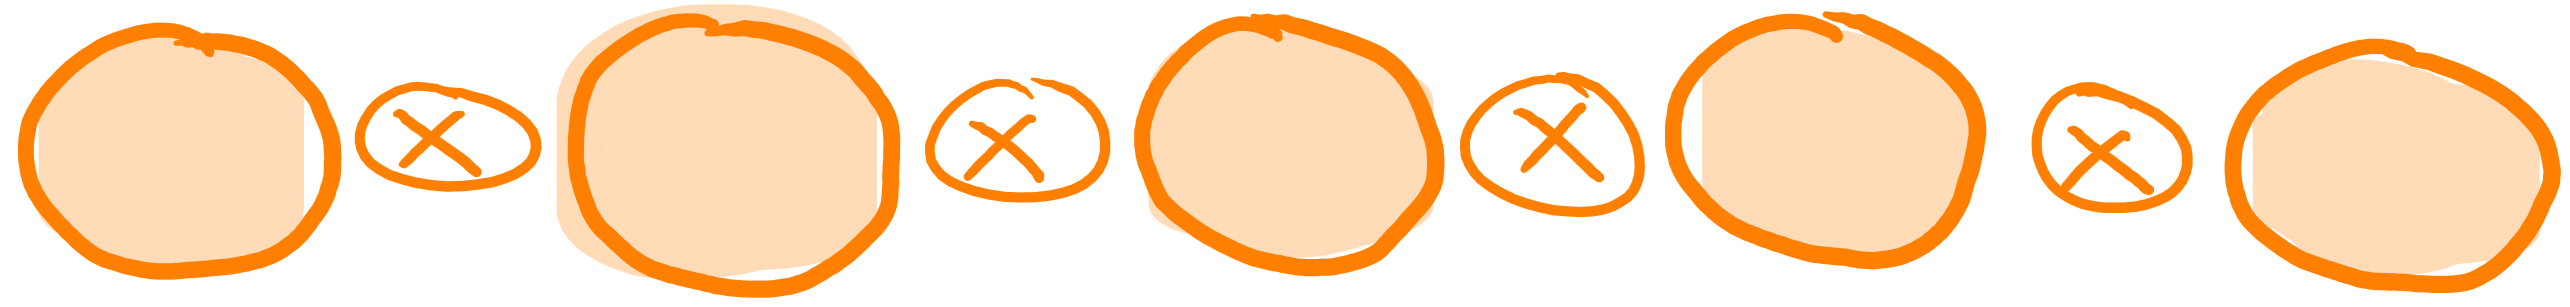
\includegraphics[scale=.2]{images/independentqubits.png}}} & 
\subfigure[]{\raisebox{.25cm}{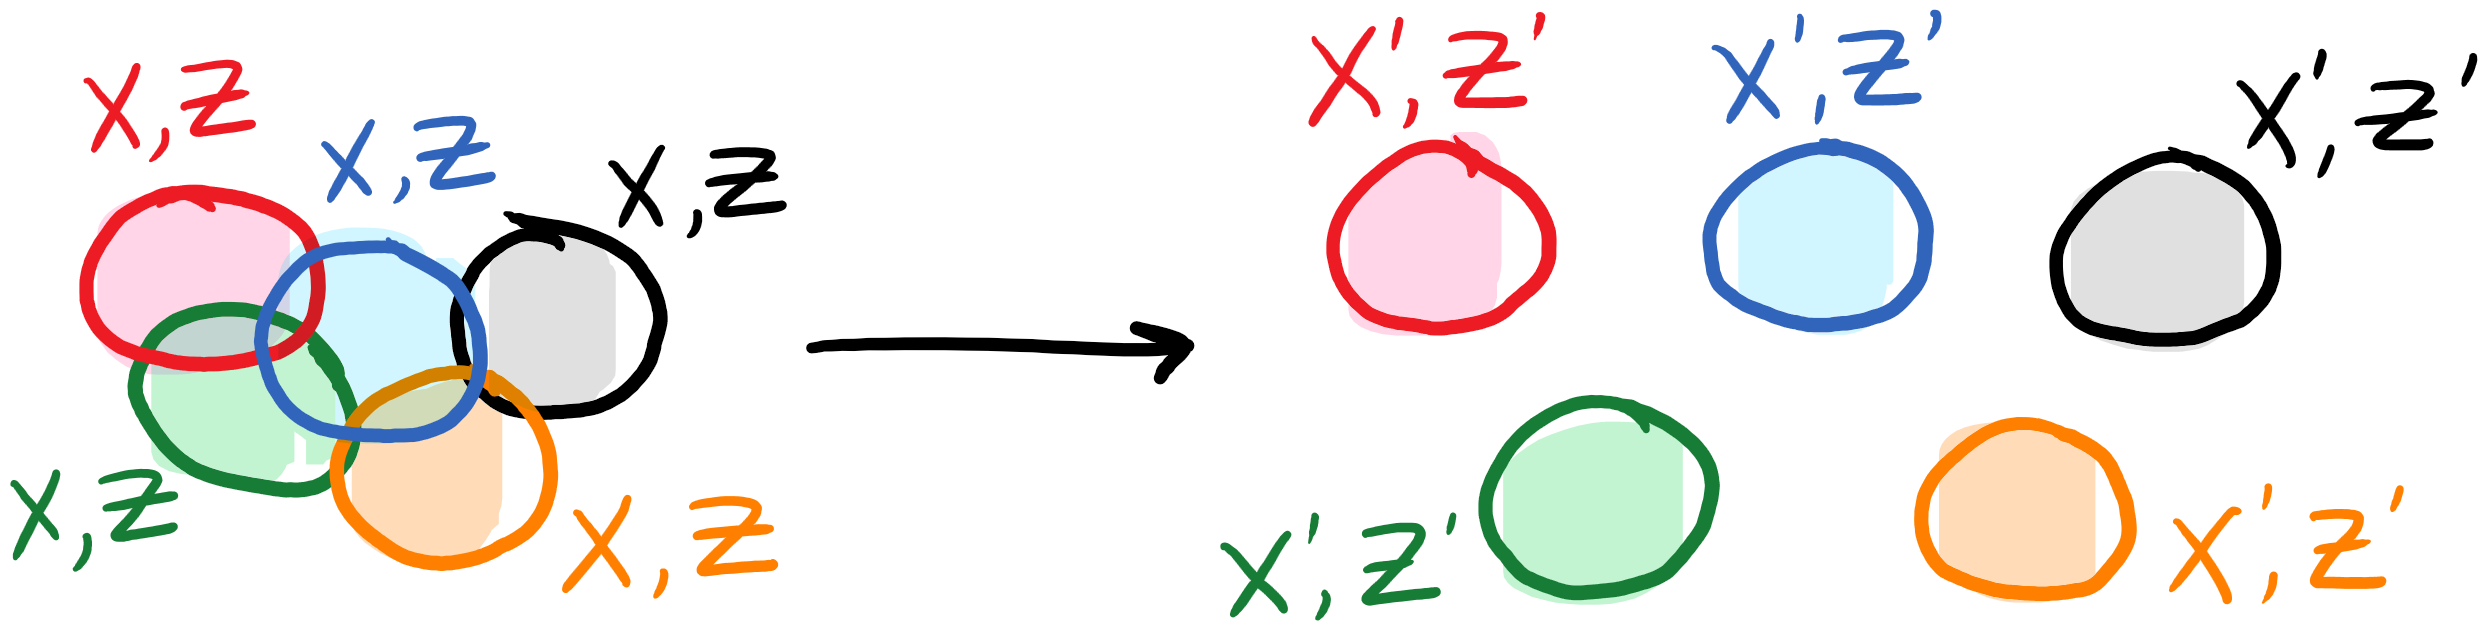
\includegraphics[scale=.25]{images/separatingqubits.png}}}
\end{tabular}
\caption{(a) A qubit is a two-dimensional system in tensor product with the rest of the space.  Qubits ``overlap" if the corresponding Pauli operators do not commute.  When their Pauli operators do commute, the qubits are in tensor product with each other (\thmref{t:whatismanyqubits}).  (b) We ask how many qubits can be packed into a $2^n$ dimensional space with small pairwise overlap.  For a lower bound, we give a randomized construction, based on the Johnson-Lindenstrauss Lemma and fermion algebra (\thmref{t:qubitpacking}).  For an upper bound, we separate qubits with small pairwise overlap, finding nearby qubits with zero overlap (\thmref{t:manynearlyindependentqubits}).} \label{f:independentandseparatingqubits}
\end{figure}

The construction in the upper bound loses a factor of~$n$, and we give an example to show that this is necessary (\lemref{t:movementlowerbound}).  Yet there is still a gap between our lower and upper bounds.  For the range of overlaps $1 / n \lesssim \epsilon \lesssim \sqrt{(\log n) / n}$, we do not know whether strictly more than $n$ qubits can be packed into $2^n$ dimensions.  

\smallskip

Given access to an experimental system, it is difficult to imagine tests for determining $\norm{[S_i, T_j]}$.  The problem is that the quantum system can be in an unknown state $\ket \psi$, and we can only learn about operators' effects on $\ket \psi$.  If $S_i$ and~$T_j$ are far from commuting, but only on a portion of the Hilbert space in which $\ket \psi$ has no support, this is undetectable.  In \secref{s:statedependent}, we therefore consider a \emph{state-dependent} overlap measure.  This is the same measure that is used in results on self-testing such as~\cite{MayersYao98chsh,McKagueYangScarani12chshrigidity}, and it is the relevant measure for applications to device-independent cryptography~\cite{Kaniewski14entropic}.  Note however that our setting differs from the usual one in self-testing, as we do not assume any a priori bipartite structure on the Hilbert space; though our results do apply to bipartite entanglement testing~\cite{ChaoReichardtSutherlandVidick16}.  

We first give a practical protocol for testing if $\norm{[S_i, T_j] \ket \psi} \approx 0$: measure $S_i$, measure $T_j$, then measure $S_i$ again and check that it gives the same result.  However, this test is not enough; we give a construction of a state and $n$ qubit operators in $< n^2$ dimensions, such that for $i \neq j$, $[S_i, T_j] \ket \psi = 0$ exactly.  Finally we give a more advanced test that efficiently checks not just pairwise commutation relationships, like $[S_i, T_j] \ket \psi \approx 0$, but also higher-order relationships like $S_i T_j U_k \ket \psi \approx U_k T_j S_i \ket \psi$.  This test can verify that the system dimension is almost~$2^n$.  


\ifx\compilefullpaper\undefined  
%\addcontentsline{toc}{section}{References}
\bibliographystyle{alpha-eprint}
\bibliography{q}

\end{document}
\fi